\chapter{Key Decisions}

\section{Mean Reversion Strategies}
Considering the current state of the art and the limited exploration of statistical arbitrage in decentralized exchanges, the objective of this project is to examine the profitability of mean reversion techniques in pairs trading and determine if they offer a viable investment opportunity. Additionally, by employing various methods to estimate the hedge ratio and effectively manage risk, we can further analyze the overall performance and appeal of the trading strategy to potential traders.
\\[5mm]
In the mean reversion strategies, the hedge ratio refers to the ratio or proportion between the positions of two assets involved in a pairs trading strategy. It determines the optimal allocation of capital between the assets to minimize risk and create a market-neutral position. The hedge ratio represents the number of units or shares of one asset that should be held for each unit or share of the other asset in order to create a balanced or hedged position. It is derived through statistical techniques such as regression analysis. The methods that are explored in this paper are the use of a Constant Hedge Ratio, Sliding Window Ordinary Least Squares, Lagged Ordinary Least Squares, the unrestricted OLS model returned by the Granger Causality Test and also the Kalman Filter. These methods are selected due to their ability to test whether underlying dynamics effect the relationships between liquidity pools, hence effecting the hedge ratio. To further see the details and implementation of each strategy, refer to Section \ref{sec:strats}.

\section{Buying and Selling}
\label{sec:buying-selling}
The process of buying and selling in traditional markets is relatively straightforward as brokers and exchanges play a crucial role in executing orders on behalf of individuals. However, when it comes to trading cryptocurrencies, the responsibility falls directly on the trader, such as myself. Therefore, it becomes essential to clearly define what buying and selling entail in the context of cryptocurrency trading.

\subsection{Buying}
Prices on Uniswap are represented as ratios for example 1 USDC = $P$ WETH. With this understanding, let's delve into the process of buying one unit of USDC/WETH on Uniswap:
\begin{itemize}
    \item Opening a Buy position:\begin{itemize}
        \item Starts with $P_{0}$ WETH
        \item Swaps the WETH for USDC, hence ends with 1 USDC
    \end{itemize}
    \item Closing a Buy position:\begin{itemize}
        \item Starts with 1 USDC
        \item Swaps the USDC for WETH, hence ends with $P_1$ WETH
    \end{itemize}
\end{itemize}
\noindent Consequently, if the price of USDC/WETH increases from the moment the buy position is opened to the time it is closed, the trader realizes a profit. On the other hand, if the price declines during this period, the trader incurs a loss.

\subsection{Selling}
Selling an asset is a more complex process compared to buying because it involves trading an asset that the trader doesn't initially possess. In traditional markets, this is facilitated by the trader borrowing the desired asset from a broker or another party. When the trader decides to close the position, they repurchase the same amount of the borrowed asset and return it to the lender, hoping that its value has declined. This borrowing and returning process is typically managed automatically by brokers and exchanges. However, in decentralized exchanges (DEXes), such mechanisms are not in place.
\\[5mm]
To simplify this process, I have opted to utilize Aave as a lending platform to borrow any required assets. It is worth noting that Aave supports only a limited range of tokens available for borrowing, namely DAI, EURS, USDC, USDT, AAVE, LINK, WBTC, and WETH. Therefore, shorting would be feasible only if I focus on liquidity pools that involve these cryptocurrencies. By leveraging Aave as a lending platform, I can access the necessary assets for shorting. The process of selling is as follows:
\begin{itemize}
    \item Opening a Sell position:\begin{itemize}
        \item Borrow 1 USDC
        \item Swaps the USDC for WETH, hence ends with $P_0$ WETH
    \end{itemize}
    \item Closing a Sell position:\begin{itemize}
        \item Starts with $P_0$ WETH
        \item Swaps the WETH for USDC, hence ends with $\frac{P_0}{P_1}$ USDC
        \item Return the borrowed USDC, leaving $\frac{P_0}{P_1} - 1$ USDC
    \end{itemize}
\end{itemize}
Consequently, if the price of USDC/WETH decreases, i.e. $P_1 < P_0$ from the moment the sell position is opened to the time it is closed, the trader realizes a profit. On the other hand, if the price increases during this period, the trader incurs a loss.
\\[5mm]
Note that this is is merely an illustrative example and does not account for any potential fees that the trader might incur.


\section{Protocols of Interest}
\subsection{Uniswap}

\subsubsection{Overview}
Uniswap is a decentralized exchange protocol built on the Ethereum blockchain. It allows users to trade ERC-20 tokens directly from their wallets without the need for intermediaries or traditional order books. Uniswap utilizes automated market-making, where liquidity providers contribute funds to liquidity pools, earning fees on trades made in the pool. The protocol employs a mathematical formula called the constant product formula to maintain balanced token ratios in the pool. When users want to make a trade, Uniswap calculates the conversion based on the pool's token ratios and executes the trade through a smart contract.

\subsubsection{Automated Market Maker (AMM) Model and Liquidity Pools}

The AMM model is a system that replaces traditional order books with liquidity pools to facilitate trading between different tokens. Automated Market Makers do this with the aid of liquidity pools. They are pools of tokens contributed by liquidity providers (LPs) to facilitate trading between different tokens within the exchange. One paper describes pools as ``a smart contract that holds at least two cryptoassets and allows trading through depositing a token of one type and thereby withdrawing tokens of the other type''~\cite{schar2021decentralized}. These liquidity pools are maintained by smart contracts on Ethereum and Liquidity Providers (LPs). Liquidity providers are individuals that voluntarily contribute an equal amount of cryptocurrencies liquidity pools, for example, in a pool for trading ETH and DAI, LPs would contribute an equal value of ETH and DAI tokens. LPs are incentivised to do provide liquidity in exchange for a share of the trading fees that occur in the liquidity pool. LPs can later withdraw their shares along with the accumulated fees. On Uniswap V3, the fee is 0.3\% on Ethereum, however they can be any of 0.01\%, 0.05\%, 0.3\%, or 1\% depending on blockchain network.

\subsubsection{Constant Product Formula}

To maintain a balanced ratio between the tokens in the pool and price any swaps, the AMM model relies on a mathematical formula called the constant product formula ($xy = k$). As trades occur, the product of the token balances remains constant. When one token's value increases, its proportion in the pool decreases, ensuring an automatic adjustment in prices. When a trade is executed, the change in prices can be described in this formula $(x + \Delta x)(y + \Delta y) = k$. Hence, after rearranging: $\Delta y = \frac{k}{x + \Delta x} - y$. Under this model, the balance of the tokens in a liquidity pool can never be depleted as the token will get infinitely more expensive as the reserves approach 0.

\begin{figure}[!htb]
    \centering
    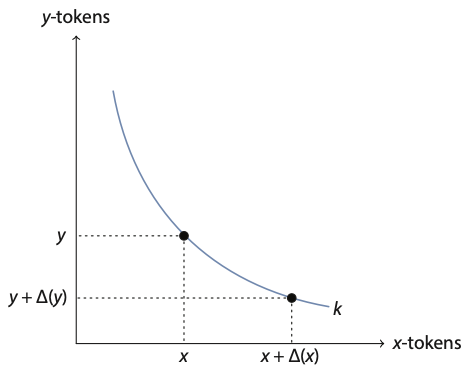
\includegraphics[width=0.5\textwidth]{background/Images/constant_product_formula.png}
    \caption{Constant Product Formula~\cite{schar2021decentralized}}
\end{figure}

\subsubsection{Slippage}

As seen in Figure \ref{fig:uniswap_lp}, we can see how the constant product formula is used in Uniswap. Uniswap also allow users to set slippage tolerance levels, which determine the maximum acceptable difference between the expected and executed prices. Slippage refers to the difference between the expected price of a trade and the executed price due to market volatility and liquidity conditions. Slippage happens because the constant product formula adjusts prices based on the ratio of tokens in the pool. As trades are executed, the token balances change, and the prices change accordingly. Thus, larger trades can cause more significant price impact, resulting in slippage.

\begin{figure}[!htb]
    \centering
    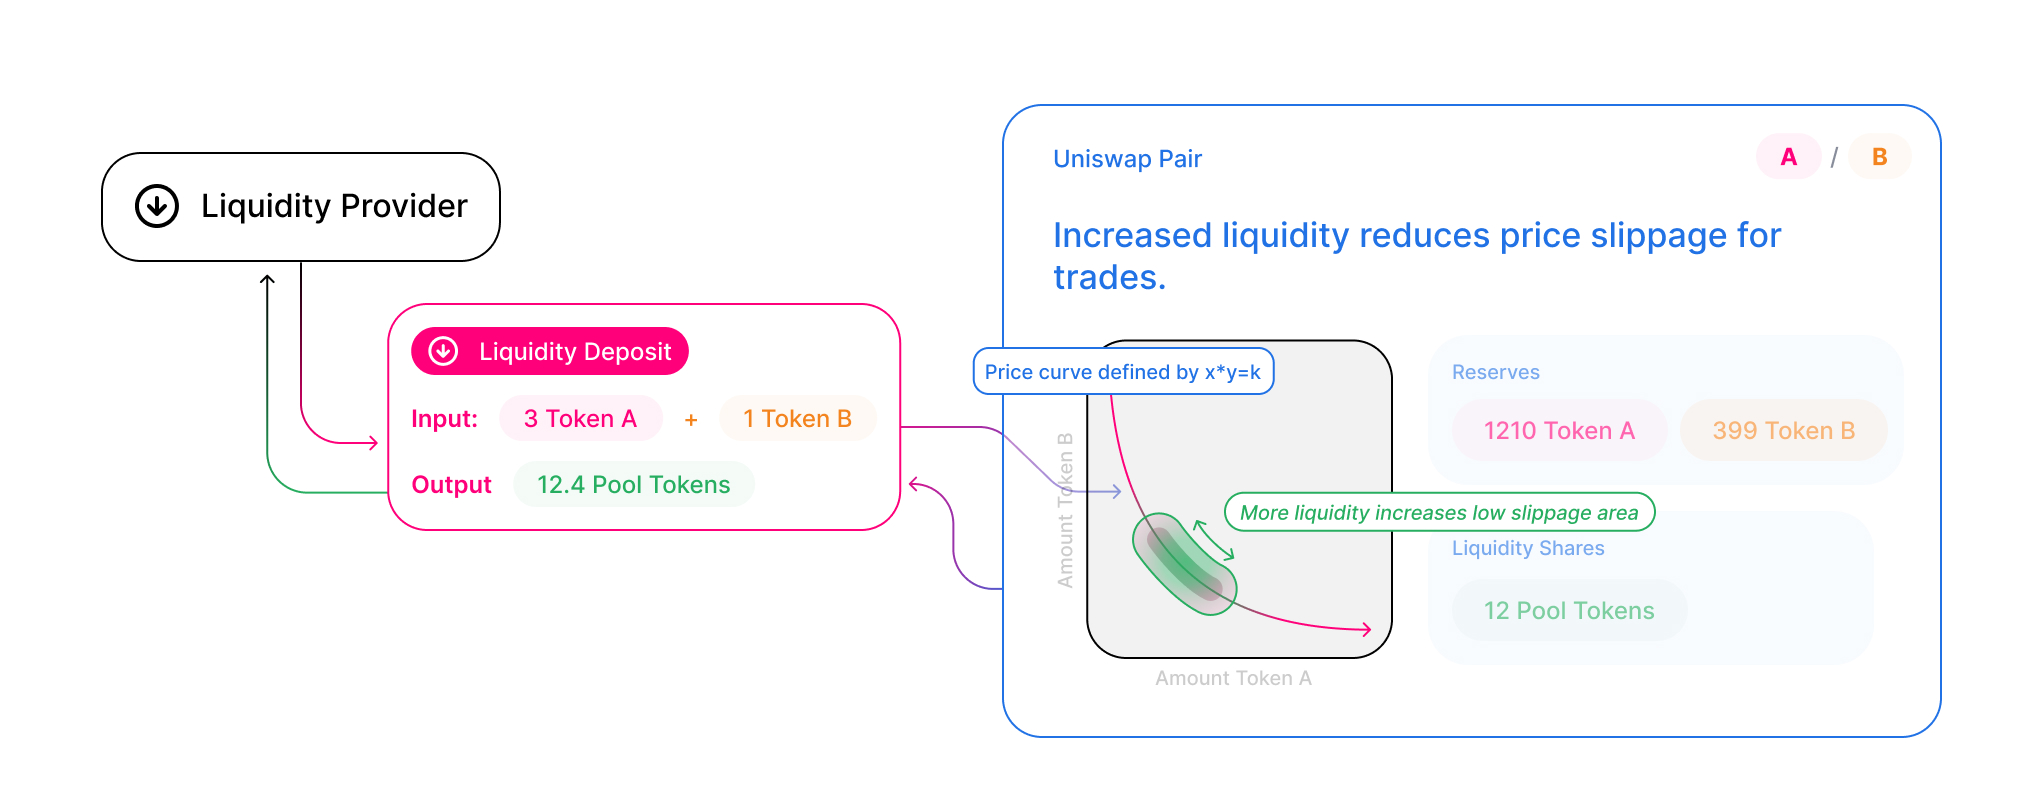
\includegraphics[width=\textwidth]{background/Images/uniswap_lp.jpeg}
    \caption{How Uniswap works~\cite{uniswap} \label{fig:uniswap_lp}}
\end{figure}

\subsection{Aave}

\subsubsection{Overview}
Aave is a decentralized lending and borrowing protocol built on the Ethereum blockchain. It enables users to lend and borrow a wide range of cryptocurrencies directly, without the need for intermediaries such as banks. Aave operates through liquidity pools and smart contracts, providing a secure, transparent, and efficient platform for decentralized finance (DeFi) activities.

Users can deposit their cryptocurrency assets into Aave's liquidity pools and earn interest on their deposits. These funds contribute to the available liquidity for borrowers. On the other hand, borrowers can use their deposited assets as collateral to borrow other assets from the pool. The amount they can borrow is determined by the value of their collateral and specific borrowing parameters set by the protocol.

\subsubsection{Liquidity Pools}

The fundamental mechanism that enables Aave's functionality of lending and borrowing is liquidity pools. Users deposit their cryptocurrency assets into Aave's liquidity pools. These assets serve as collateral and contribute to the overall liquidity of the protocol. The deposited assets in the liquidity pools create reserves of available liquidity. These reserves are utilized to fulfill borrowing demands from other users within the Aave ecosystem.

\subsubsection{Lending and Borrowing}

Lending works by lenders depositing their cryptocurrency assets into Aave's liquidity pools. These assets act as collateral and are represented by interest-bearing tokens called aTokens. The aTokens represent the user's share of the deposited assets. Interest is earnt immediately and is accrued in real-time and reflected in an increase in the quantity of aTokens held by the depositor.

Borrowing works by borrowers using their deposited assets as collateral to borrow other assets from the liquidity pools. The value of the collateral determines the borrowing capacity. The borrowing capacity is calculated by paramters set by Aave, one of which is the maximum loan-to-value (LTV) ratio. Once the borrower requests a loan, if the borrower's collateral meets the necessary requirements, they can proceed with the loan and the borrowed funds are transferred to the borrower's wallet. In addition to this, borrowers pay interest on the borrowed amount based on the prevailing interest rates. Aave offers both variable and stable interest rates for borrowers. Variable rates fluctuate based on market dynamics, while stable rates remain fixed. This flexibility allows users to choose the borrowing option that best suits their needs. The interest on a loan is accrued in real-time, second by second, and the borrower decides when to repay it, as long as the loan is safe from liquidation. Liquidation is what happens if the value of a borrower's collateral falls below the liquidation threshold due to market volatility or other factors, the collateral may be liquidated. Liquidators can purchase the collateral at a discounted price to ensure the solvency of the liquidity pool.

\section{Liquidity Pool Pairs of Interest}
\label{sec:liquidity-pools}
As previously mentioned, Uniswap is a decentralized exchange protocol that facilitates swapping of cryptocurrencies through the use of liquidity pools. One of the remarkable features of Uniswap is its support for even the smallest cryptocurrencies. In fact, it currently possesses 12,182 liquidity pools, as obtained via the Uniswap V3 subgraph. The subgraph provides valuable insights into the liquidity pools within the Uniswap ecosystem.
\\[5mm]
Table \ref{tab:liquidity_pools} showcases the diversity of these pools. Some pools exhibit high trading volumes, indicating significant activity and demand for those specific pairs. On the other hand, there are also pools with zero liquidity, which could be attributed to various reasons. It could be due to a lack of demand for one of the token pairs offered in the pool, or it may indicate that the pool is relatively new and has not attracted significant participation yet.
\\[5mm]
To enhance the chances of successful swaps and maximize potential profitability, my strategy is centered on liquidity pools with a trading volume surpassing \$10,000,000 (or \$10 million) and pools that include tokens supported by Aave. Additionally, I exclude any liquidity pools that do not involve WETH, which is a tokenized form of ETH (Ethereum's native cryptocurrency). WETH's key advantage lies in its ability to align with ERC-20 standards, enabling broader compatibility and utilization across the Ethereum ecosystem.

\begin{table}[!ht]
    \centering
    \begin{tabular}{|p{7em}|p{4em}|p{4em}|p{10em}|p{\linewidth / 6}|p{4em}|}
    \hline
        pool address & token0 & token1 & volume in USD & created at timestamp & feetier \\ \hline
        \truncate{7em}{0x88e6a0c2ddd26feeb64f039a2c41296fcb3f5640} & USDC & WETH & \truncate{10em}{375230561243.465} & 1620250931 & 500 \\ \hline
        \truncate{7em}{0x8ad599c3a0ff1de082011efddc58f1908eb6e6d8} & USDC & WETH & \truncate{10em}{70454095868.0967} & 1620169800 & 3000 \\ \hline
        \truncate{7em}{0x11b815efb8f581194ae79006d24e0d814b7697f6} & WETH & USDT & \truncate{10em}{62385006691.8387} & 1620251172 & 500 \\ \hline
        \truncate{7em}{0x3416cf6c708da44db2624d63ea0aaef7113527c6} & USDC & USDT & \truncate{10em}{57192593471.8346} & 1636825557 & 100 \\ \hline
        \truncate{7em}{0x4585fe77225b41b697c938b018e2ac67ac5a20c0} & WBTC & WETH & \truncate{10em}{49170385539.9928} & 1620246230 & 500 \\ \hline
        \truncate{7em}{0x4e68ccd3e89f51c3074ca5072bbac773960dfa36} & WETH & USDT & \truncate{10em}{30135014933.0963} & 1620232628 & 3000 \\ \hline
        \truncate{7em}{0x60594a405d53811d3bc4766596efd80fd545a270} & DAI & WETH & \truncate{10em}{26075053939.434} & 1620237823 & 500 \\ \hline
        \truncate{7em}{0xcbcdf9626bc03e24f779434178a73a0b4bad62ed} & WBTC & WETH & \truncate{10em}{21870989841.1326} & 1620158974 & 3000 \\ \hline
        \truncate{7em}{0x5777d92f208679db4b9778590fa3cab3ac9e2168} & DAI & USDC & \truncate{10em}{16143305036.8948} & 1636771503 & 100 \\ \hline
        \truncate{7em}{0x7858e59e0c01ea06df3af3d20ac7b0003275d4bf} & USDC & USDT & \truncate{10em}{15473402409.0591} & 1620159478 & 500 \\ \hline
        \truncate{7em}{0x99ac8ca7087fa4a2a1fb6357269965a2014abc35} & WBTC & USDC & \truncate{10em}{12568187132.1649} & 1620241995 & 3000 \\ \hline
        \truncate{7em}{0xc2e9f25be6257c210d7adf0d4cd6e3e881ba25f8} & DAI & WETH & \truncate{10em}{12519316091.9979} & 1620159368 & 3000 \\ \hline
        \truncate{7em}{0xe0554a476a092703abdb3ef35c80e0d76d32939f} & USDC & WETH & \truncate{10em}{9381529300.20357} & 1636926269 & 100 \\ \hline
        \truncate{7em}{0x6c6bc977e13df9b0de53b251522280bb72383700} & DAI & USDC & \truncate{10em}{7219493916.70291} & 1620158293 & 500 \\ \hline
        \truncate{7em}{0xac4b3dacb91461209ae9d41ec517c2b9cb1b7daf} & APE & WETH & \truncate{10em}{6621032721.87519} & 1647516735 & 3000 \\ \hline
        \truncate{7em}{0x8c54aa2a32a779e6f6fbea568ad85a19e0109c26} & FEI & USDC & \truncate{10em}{6206853090.73714} & 1621839430 & 500 \\ \hline\hline
        \truncate{7em}{0x53dd58b3143f428b449c16dd5706cee7d7bcf408} & sOHM & gOHM & 0 & 1652914688 & 10000 \\ \hline
        \truncate{7em}{0xbc90c4de85a4b559060cb28abfd4476ab6711f1a} & SHIB & NSTIC & 0 & 1652910391 & 100 \\ \hline
        \truncate{7em}{0xaa1297b08d0035f06309c1bfa36582c24b4ae361} & BUSD & DPC & 0 & 1674655715 & 100 \\ \hline
        \truncate{7em}{0x75087e5330c97f7ec7f716c6566f214cb0029f6a} & DAI & ICAP & 0 & 1652899566 & 10000 \\ \hline
        \truncate{7em}{0xc65a680191bd17a18c957c8aa2d1155ed2322792} & stkAAVE & FRAX & 0 & 1652817927 & 10000 \\ \hline
        \truncate{7em}{0x94589b18b95b355ee9a900f3df671b431779e20a} & VVV & SOL & 0 & 1674701603 & 10000 \\ \hline
        \truncate{7em}{0xf42f0def92337b6a83753c9fae6d579f7d67aaa9} & APEFI & ApeUSD & 0 & 1652808878 & 3000 \\ \hline
        \truncate{7em}{0xb9ba65f1568b318ffc1879a4a6368ef2b5ac96b8} & FRAX & ApeUSD & 0 & 1652808680 & 500 \\ \hline
        \truncate{7em}{0x1dfb167f1ba47f3bf835eb60a9317b4601925642} & GHD & WETH & 0 & 1652784327 & 3000 \\ \hline
    \end{tabular}
    \caption{A selection of liquidity pools on Uniswap \label{tab:liquidity_pools}}
\end{table}

\subsection{Correlated and Cointegrated Liquidity Pools}
Once the liquidity pools of interested in have been identified, it is crucial to filter the pool pairs based on their correlation. This is because correlated pairs tend to exhibit similar pricing movements thus would be possible to apply the mean reversion trading strategies. However, it is important to strike a balance between a highly correlated pair and a low correlated pair, as excessively high correlation can result in minimal price deviations, leading to fees that exceed the deviations and resulting in overall losses instead of profits. To address this, I have set a condition where the correlation coefficient ($\rho$) should fall within the range of $0.992 \leq \rho \leq 0.997$. Figure \ref{fig:correlationMatrix} shows the correlation matrix of the liquidity pools that meet the initial requirement of having a volume greater than \$10 million volume ratio and include WETH. Notably, the pools associated with tokens aiming to be pegged to the US Dollar, such as USDT, USDC, and DAI, exhibit the expected high correlation with each other. However, an exception is observed with pool 0xe0554a476a092703abdb3ef35c80e0d76d32939f, which exhibits a lower correlation with other liquidity pools containing these stable coins. Consequently, this lower correlation opens up additional avenues for potential arbitrage opportunities within the pool.
\begin{figure}[!htb]
    \centering
    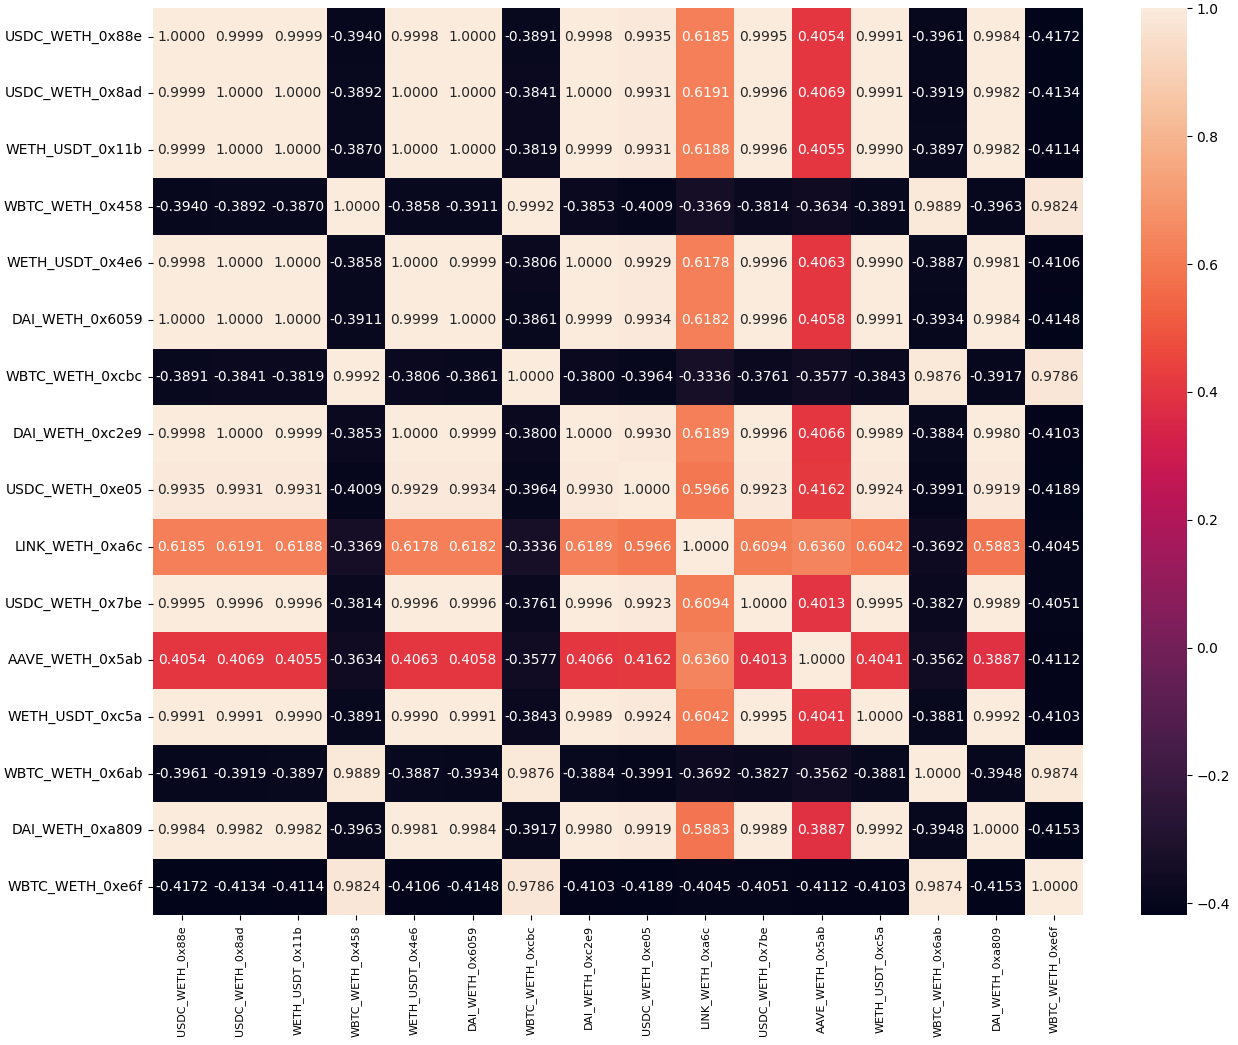
\includegraphics[width=\textwidth]{project/Images/correlationMatrix.png}
    \caption{Correlation Matrix of the Liquidity Pools that meet the \$10 million volume and include WETH \label{fig:correlationMatrix}}
\end{figure}
\\[5mm]
To determine which liquidity pools are cointegrated, I employed the Engle-Granger approach. The Engle-Granger test for cointegration involves several steps. Firstly, a unit root test is performed individually on each time series using methods like the Augmented Dickey-Fuller (ADF) test or the Phillips-Perron (PP) test. These tests assess whether the time series are stationary or exhibit unit roots (non-stationary) individually. For cointegration to hold, both time series must be non-stationary.
\\[5mm]
Once it is established that both time series are non-stationary, an estimation of the cointegration equation is derived. Typically, a linear regression model is employed to capture the long-term relationship between the time series variables. This equation provides an understanding of how the variables are linked over a long period.
\\[5mm]
Subsequently, a unit root test is conducted on the residuals obtained from the regression analysis. If the residuals are stationary (indicating the absence of unit roots), it suggests the presence of cointegration between the time series. This implies that the variables move together in the long run, even if short-term deviations occur.
\\[5mm]
By following the aforementioned sequence of steps in the Engle-Granger test, it enables us to determine which liquidity pools demonstrate cointegration, thereby emphasizing their interconnectedness and mutual relationship over time. The outcome of the cointegration tests for all possible combinations of liquidity pools is presented in Table \ref{tab:coin_pools}. This table provides a comprehensive list of the liquidity pool pairs along with the results of their respective cointegration tests and the correlation coefficient of each combination.
\begin{table}[!ht]
    \centering
    \begin{adjustwidth}{-1in}{-0.9in}
        \begin{tabular}{|p{12em}|p{12em}|p{5em}|p{4.2em}|p{4.2em}|p{4.2em}|p{3.5em}|}\hline
            pool1 & pool2 & t-statistic of unit-root test on residuals & \multicolumn{3}{|c|}{Critical Values} & Corr Coeff\\[-1ex]\cline{4-6}
            &   &   & 1\% & 5\% & 10\% & \\\hline
            \truncate{12em}{USDC\_WETH\_0x88e6a0c2ddd26feeb64f039a2c41296fcb3f5640} & \truncate{12em}{USDC\_WETH\_0xe0554a476a092703abdb3ef35c80e0d76d32939f} & -11.306176 & -3.898069 & -3.337038 & -3.045081 & 0.99347\\\hline
            \truncate{12em}{USDC\_WETH\_0x8ad599c3a0ff1de082011efddc58f1908eb6e6d8} & \truncate{12em}{USDC\_WETH\_0xe0554a476a092703abdb3ef35c80e0d76d32939f} & -11.210146 & -3.898082 & -3.337046 & -3.045086 & 0.99307\\\hline
            \truncate{12em}{WETH\_USDT\_0x11b815efb8f581194ae79006d24e0d814b7697f6} & \truncate{12em}{USDC\_WETH\_0xe0554a476a092703abdb3ef35c80e0d76d32939f} & -10.010746 & -3.898069 & -3.337038 & -3.045081 & 0.99315\\\hline
            \truncate{12em}{WETH\_USDT\_0x4e68ccd3e89f51c3074ca5072bbac773960dfa36} & \truncate{12em}{USDC\_WETH\_0xe0554a476a092703abdb3ef35c80e0d76d32939f} & -9.913205 & -3.898081 & -3.337045 & -3.045085 & 0.99291\\\hline
            \truncate{12em}{DAI\_WETH\_0x60594a405d53811d3bc4766596efd80fd545a270} & \truncate{12em}{USDC\_WETH\_0xe0554a476a092703abdb3ef35c80e0d76d32939f} & -11.395276 & -3.898069 & -3.337038 & -3.045081 & 0.99338\\\hline
            \truncate{12em}{DAI\_WETH\_0xc2e9f25be6257c210d7adf0d4cd6e3e881ba25f8} & \truncate{12em}{USDC\_WETH\_0xe0554a476a092703abdb3ef35c80e0d76d32939f} & -10.418722 & -3.89831 & -3.337173 & -3.045174 & 0.99298\\\hline
            \truncate{12em}{USDC\_WETH\_0xe0554a476a092703abdb3ef35c80e0d76d32939f} & \truncate{12em}{WETH\_USDT\_0xc5af84701f98fa483ece78af83f11b6c38aca71d} & -9.7789 & -3.901414 & -3.338902 & -3.046374 & 0.99243\\\hline
        \end{tabular}
    \end{adjustwidth}
    \caption{Cointegration test on Liquidity Pool pairs \label{tab:coin_pools}}
\end{table}
\\[5mm]
\noindent Based on the results obtained, we focus our further investigation solely on the pairs of liquidity pools that exhibit cointegration under a 1\% confidence level. This filtering process allows us to narrow down our analysis to those pairs where a long-term relationship exists, suggesting that they move together in a concerted manner.
\\[5mm]
By concentrating on the cointegrated pairs, we can delve deeper into exploring their dynamics, assessing their behavior, and leverage the interconnectedness between these liquidity pools. This approach enables us to prioritize our analysis and concentrate on the most relevant liquidity pool combinations that offer potential opportunities for profitable trading or other related activities.



